\documentclass{beamer}
\setbeamertemplate{navigation symbols}{} % eliminate navigation bar
\usetheme{CambridgeUS}

\usefonttheme{structurebold}
% Arch Linux Color Theme
\definecolor{arch}{RGB}{23,147,209}
\usecolortheme[named=arch]{structure}
\usecolortheme{whale}
\setbeamercolor{frametitle}{bg=arch!80!black}
\setbeamercolor{title}{bg=arch!90!black}

%% SET BEAMER TEMPLATE
%\setbeamertemplate{headline}

\usepackage{lmodern}
\usepackage{ngerman}
\usepackage[latin1]{inputenc}
\usepackage[naustrian,ngerman]{babel}

\usepackage{listings}
\lstset{basicstyle=\tiny\ttfamily,
  frame=single}

\beamersetuncovermixins{\opaqueness<1>{25}}{\opaqueness<2->{15}}


%% META INFORMATION ABOUT DOCUMENT
% \title[short]{long}
% short argument is used in places where there is little space
% long is used on the title slide

\title[Impedanzspektrometer]{mini Impedanzspektrometer mit dem AD5933}
\subtitle{Bachelorarbeit SS2014}
\institute[]{Institut f�r Mikroelektronik und Mikrosensorik \\ Johannes-Kepler-Universit�t Linz}

\subject{AD5933 Impedanzspektrometer}

% ENTER YOUR NAME, SHORT VERSION FOR FOOTER
\author[Feichtinger]{Peter Feichtinger\texorpdfstring{\\}{, } Betreuer: DI Stefan Clara} % Variante: \and

\date{10. Juli 2014}


\begin{document}

%% TITLE PAGE
\begin{frame}
  \titlepage
\end{frame}

% for longer presentations table of contents is useful
% \begin{frame}
%    \frametitle{Outline} 
%    \tableofcontents          % optional: [pausesections]
% \end{frame}


\section{Stand der Bachelorarbeit}  % always defined outside a frame, optional short argument
\begin{frame}[t]
  \frametitle{Hardware}
  
  \begin{itemize}
    \item Externes Analog-Frontend zum AD5933 mit 4-Leiter Messung
    \item Analog-Multiplexer f�r mehrere Ausg�nge
    \item Austauschbare Kalibrierwiderst�nde
    %\item Platz f�r Ethernet Schnittstelle und USB-Host
  \end{itemize}
  
  \vspace{1em}
  \centering
  \only<1>{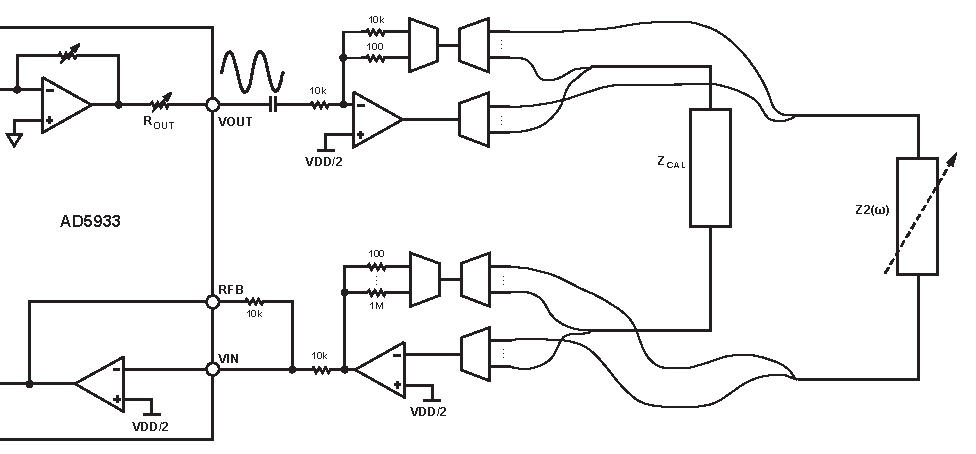
\includegraphics[height=11.5em]{bilder/schem_afe.pdf} \\
    \footnotesize{Schaltung des Analog-Frontend} }
  \only<2>{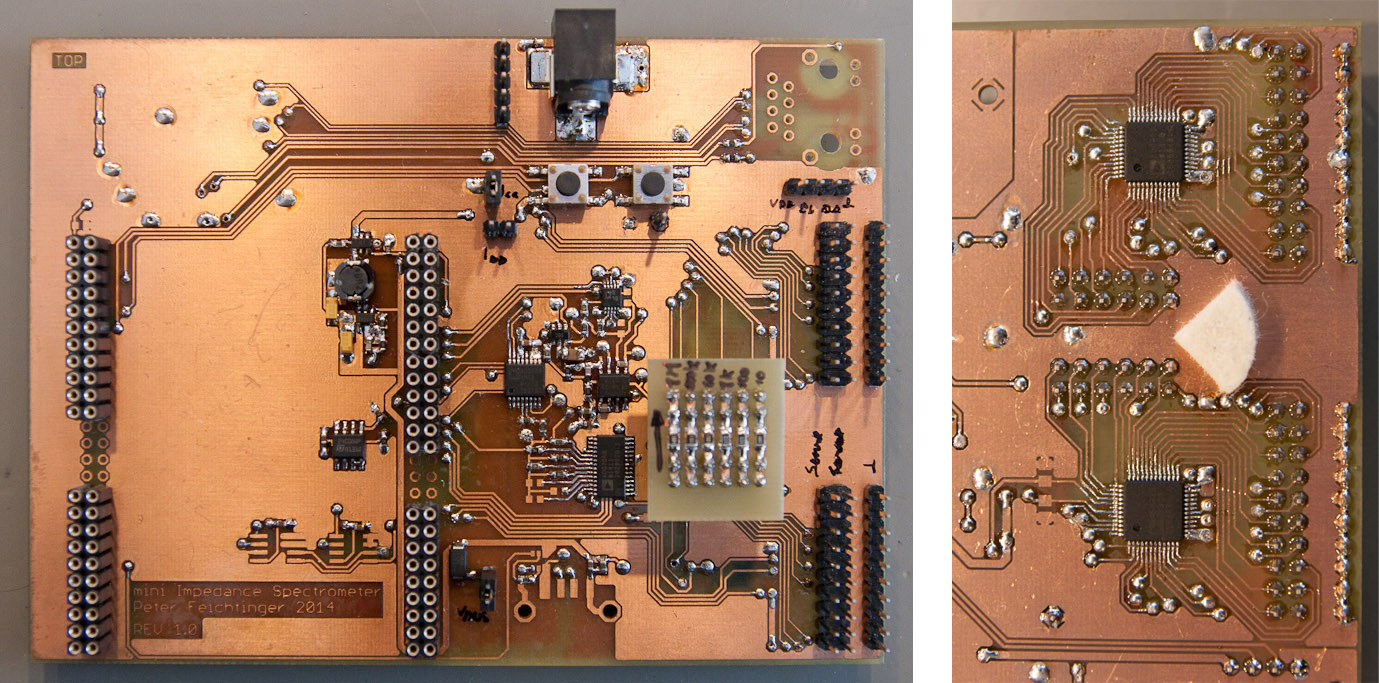
\includegraphics[height=11.5em]{bilder/pcb_rev1.jpg} \\
    \footnotesize{Erste Version der Platine} }
\end{frame}

% \pause can be used to uncover elements later
% doesn't work with align

% allowframebreaks, use rarely


\begin{frame}[c,fragile]
  \frametitle{Software}
  
  \begin{columns}
    \begin{column}{0.5\textwidth}
      \begin{itemize}
        \item Konfiguration �ber Konsoleninterface
        \item Auslesen der Werte in verschiedenen Formaten
        \item MATLAB Funktionen zur automatisierten Steuerung
      \end{itemize}
      \vspace{2cm}
    \end{column}
    
    \begin{column}{0.45\textwidth}
      \begin{lstlisting}
board set --start=10k --stop=20k
board set --steps=10 --voltage=400
board calibrate 100
OK
board start 0
OK
board read
Frequency Magnitude Angle
10000 11.5255 1.10659
11000 14.0605 1.17955
12000 18.1948 1.13351
13000 24.6496 1.04903
14000 35.7221 0.883436
15000 54.9023 0.512685
16000 68.6387 -0.185134
17000 52.3116 -0.825151
18000 36.2655 -1.12627
19000 27.0367 -1.27099
20000 21.4698 -1.35018
      \end{lstlisting}
    \end{column}
  \end{columns}
\end{frame}


\begin{frame}[c]
  \frametitle{Ausblick}
  
  \begin{columns}
    \begin{column}{0.5\textwidth}
      \begin{itemize}
        \item Robusteres Analog-Frontend
        \item Vergleichsmessungen mit Agilent 4294A
        \item Genauigkeit untersuchen
        \item Autoranging und Ethernet Schnittstelle implementieren
      \end{itemize}
      \vspace{2cm}
    \end{column}
    
    \begin{column}{0.45\textwidth}
      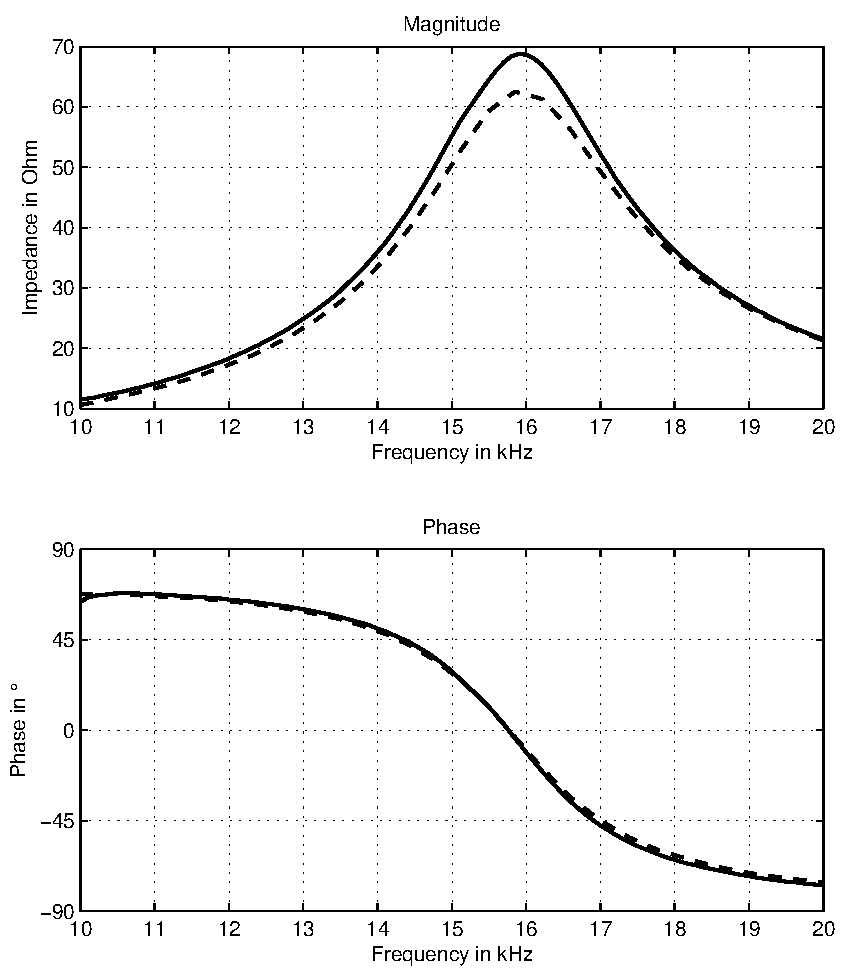
\includegraphics[height=16em]{bilder/lcp_fail.pdf}
    \end{column}
  \end{columns}
\end{frame}


%\begin{frame}
  %\centering
  %Vielen Dank f�r Ihre Aufmerksamkeit!
%\end{frame}


\end{document}